\documentclass[a4paper,12pt]{article}

\usepackage[utf8]{inputenc}
\usepackage[T1]{fontenc}
\usepackage{amsmath,amssymb}
\usepackage{geometry}
\usepackage{graphicx}
\usepackage{minted}

\geometry{margin=2.5cm}

\title{Implementacija redkih matrik in metode SOR}
\author{Matej Rupnik}
\date{\today}

\begin{document}

\maketitle

\section{Opis problema}

Obravnavamo reševanje linearnega sistema

\[
A x = b,
\]

\noindent kjer je \(A \in \mathbb{R}^{n \times n}\) razpršena matrika. Ker je pri takšnih matrikah večina elementov enaka nič, klasična gosta predstavitev matrike ni učinkovita ne prostorsko ne računsko. Zato shranjujemo le neničelne elemente in njihove indekse.

\medskip

\noindent Za reševanje sistema uporabimo iterativno metodo SOR (Successive Over-Relaxation), ki predstavlja razširitev Gauss--Seidlove metode z relaksacijskim parametrom \(\omega\). Pri izbiri

\[
\omega = 1
\]

\noindent dobimo Gauss--Seidlovo metodo, medtem ko vrednosti

\[
0 < \omega < 1
\]

\noindent predstavljajo podrelaksacijo, vrednosti

\[
1 < \omega < 2
\]

\noindent pa nadrelaksacijo, ki lahko pospeši konvergenco metode.

\noindent Iteracije ustavimo, ko velja

\[
\|Ax^{(k)} - b\|_\infty < \delta.
\]

\noindent Metodo nato uporabimo pri fizikalni vložitvi grafov v ravnino oziroma prostor.

\newpage

\section{Redka matrika}

Razpršene matrike predstavimo s strukturo tipa \texttt{RedkaMatrika}:

\begin{minted}{julia}
struct RedkaMatrika
    V::Vector{Vector{Float64}}
    I::Vector{Vector{Int}}
    n::Int
end
\end{minted}

\noindent Vsaka vrstica matrike je predstavljena z dvema seznamoma:
\begin{itemize}
    \item \texttt{V[i]} vsebuje neničelne vrednosti v vrstici \(i\),
    \item \texttt{I[i]} vsebuje pripadajoče stolpčne indekse.
\end{itemize}

\noindent Takšna predstavitev ustreza formatu LIL (List of Lists), ki je posebej primeren za iterativne metode in množenje matrike z vektorjem.

\noindent Implementirali smo osnovne operacije nad matrikami:
\begin{itemize}
    \item indeksiranje elementov,
    \item spreminjanje vrednosti,
    \item množenje z vektorjem,
    \item seštevanje, odštevanje in množenje s skalarjem,
    \item pretvorbo med gosto in razpršeno predstavitvijo.
\end{itemize}

\noindent Najpomembnejša operacija za metodo SOR je množenje matrike z vektorjem:

\begin{minted}{julia}
function Base.:*(A::RedkaMatrika, x::Vector{Float64})
    y = zeros(A.n)

    for i in 1:A.n
        for (val, j) in zip(A.V[i], A.I[i])
            y[i] += val * x[j]
        end
    end

    return y
end
\end{minted}

\noindent Ker upoštevamo le neničelne elemente, je izračun učinkovitejši kot pri gosti predstavitvi matrike.

\section{SOR metoda}

Za reševanje sistema

\[
A x = b
\]

\noindent uporabimo iterativno metodo SOR. Metoda v vsaki iteraciji zaporedoma posodobi komponente vektorja \(x\), pri čemer uporabi trenutno najboljši približek rešitve. Iteracija se ustavi, ko velja

\[
\|Ax^{(k)} - b\|_\infty < \delta.
\]

\noindent Implementacija metode:

\begin{minted}{julia}
function sor(A::RedkaMatrika,
             b::Vector{Float64},
             omega::Float64=1.0,
             tol=1e-10)

    max_iterations = 10_000
    n, _ = size(A)
    x = zeros(n)

    for iteration in 1:max_iterations
        for row in 1:n
            diagonal_entry, row_sum = rowTerms(A, row, x)

            x[row] = (1 - omega) * x[row] +
                     (omega / diagonal_entry) *
                     (b[row] - row_sum)
        end

        residual = A * x - b

        if norm(residual, Inf) < tol
            return x, iteration
        end
    end

    error("Convergence not achieved")
end
\end{minted}

\noindent Za posamezno vrstico matrike posebej ločimo diagonalni element od ostalih prispevkov. To omogoča pomožna funkcija \texttt{rowTerms}, ki rekonstruira prispevek trenutne vrstice pri posodobitvi komponente vektorja \(x\).

\newpage

\section{Fizikalna vložitev grafov}

Metodo SOR uporabimo tudi pri fizikalni vložitvi grafov v ravnino. Vozlišča grafa obravnavamo kot točke, povezane z vzmetmi, njihove lege pa določimo iz ravnotežnih pogojev sistema. To vodi do reševanja razpršenega linearnega sistema z Laplaceovo matriko grafa, ki je za večino grafov redka.

\subsection{Krožna lestev}

\begin{figure}[h]
    \centering
    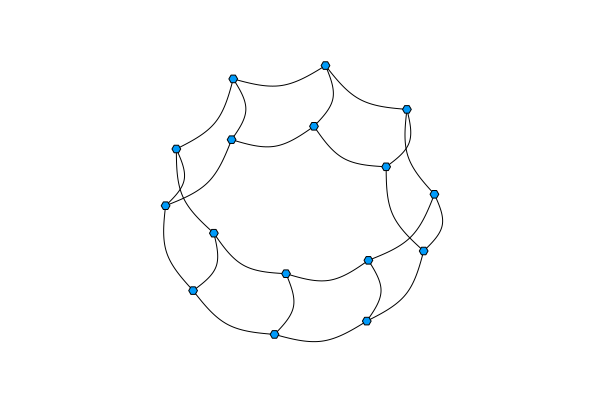
\includegraphics[width=0.45\textwidth]{krozna_lestev.png}
    \caption{Začetna struktura krožne lestve.}
\end{figure}

\begin{figure}[h]
    \centering
    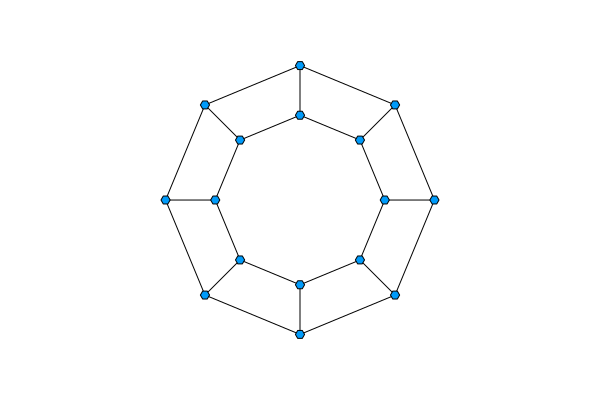
\includegraphics[width=0.45\textwidth]{vlozena_krozna_lestev.png}
    \caption{Vložitev krožne lestve po uporabi metode SOR.}
\end{figure}

\newpage
\subsection{Vložitev 2D mreže}

\begin{figure}[h]
    \centering
    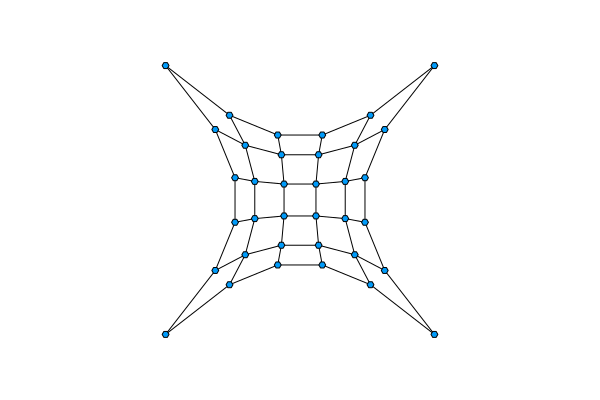
\includegraphics[width=0.5\textwidth]{vlozena_2d_mreza.png}
    \caption{Fizikalna vložitev 2D mreže.}
\end{figure}


\section{Testiranje}

Pravilnost implementacije smo preverili z avtomatskimi testi za podatkovni tip \texttt{RedkaMatrika} in metodo SOR.

\noindent Pri redki matriki smo preverili:
\begin{itemize}
    \item pretvorbo med gosto in razpršeno predstavitvijo,
    \item indeksiranje elementov,
    \item množenje z vektorjem,
    \item osnovne aritmetične operacije.
\end{itemize}

\noindent Pri metodi SOR smo preverili:
\begin{itemize}
    \item konvergenco na diagonalno dominantnih sistemih,
    \item pravilnost glede na referenčno rešitev,
    \item vpliv parametra \(\omega\),
    \item ustavitveni pogoj,
    \item obnašanje pri ničelnem diagonalnem elementu.
\end{itemize}

\newpage

\section{Rezultati}

Implementacija je pravilno rešila vse testne sisteme in dosegla zahtevano toleranco.

\noindent Posebej smo opazovali vpliv parametra \(\omega\) na hitrost konvergence. Pokazalo se je, da ustrezna izbira nadrelaksacije lahko bistveno zmanjša število iteracij.

\begin{figure}[h]
    \centering
    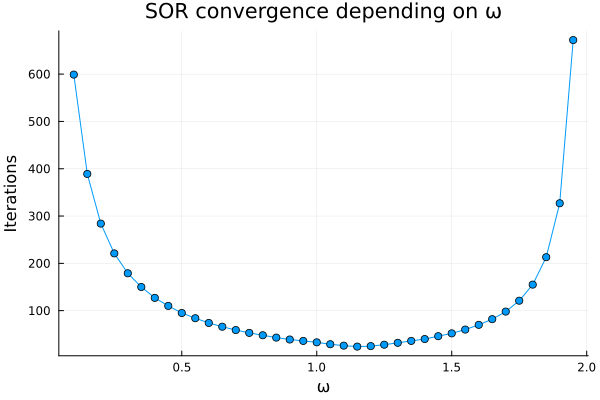
\includegraphics[width=0.6\textwidth]{optimal_omega.png}
    \caption{Vpliv parametra \(\omega\) na število iteracij metode SOR.}
\end{figure}

\noindent V naših primerih se je optimalna vrednost parametra pojavila pri približno

\[
\omega \approx 1.1 - 1.2,
\]

\noindent kjer je metoda konvergirala najhitreje.

\end{document}